\documentclass[a4paper,11pt]{article}
\usepackage{amssymb}
\usepackage[polish]{babel}
\usepackage[utf8]{inputenc}
\usepackage[T1]{fontenc}
\usepackage{array}
\usepackage{graphicx}
\usepackage{anysize}
\usepackage{enumerate}
\usepackage{times}
\usepackage{geometry}
\usepackage{amsthm}
\usepackage{pgfplots}
\usepackage{sidecap}
\usepackage{wrapfig}
\usepackage[format=hang,font=small,labelfont=bf]{caption}


\usepackage[intlimits]{amsmath}
\marginsize{3cm}{3cm}{1.5cm}{1.5cm}
\sloppy

\begin{document}
\begin{table}[ht]
\centering
\hspace*{-1cm}
\begin{tabular}{lllllll}
\cline{1-6}
\multicolumn{1}{|c|}{\begin{tabular}[c]{@{}c@{}}EAIiIB\\ Informatyka\end{tabular}}              & \multicolumn{2}{l|}{\begin{tabular}[c]{@{}l@{}}Aleksander Lisiecki\\ Natalia Materek\end{tabular}}                                                                                                & \multicolumn{1}{c|}{\begin{tabular}[c]{@{}c@{}}Rok\\ II\end{tabular}}          & \multicolumn{1}{c|}{\begin{tabular}[c]{@{}c@{}}Grupa\\ 2\end{tabular}}            & \multicolumn{1}{c|}{\begin{tabular}[c]{@{}c@{}}Zespół\\ 6\end{tabular}}      &  \\ \cline{1-6}
\multicolumn{1}{|c|}{\begin{tabular}[c]{@{}c@{}}Pracownia\\ FIZYCZNA\\ WFiIS AGH\end{tabular}} & \multicolumn{4}{l|}{\begin{tabular}[c]{@{}l@{}}Temat:\\ \textbf{\textit{Wahadło fizyczne}} \end{tabular}}                                                                                                                                                                                                                                            & \multicolumn{1}{c|}{\begin{tabular}[c]{@{}c@{}}Nr ćwiczenia:\\ 1\end{tabular}} &  \\ \cline{1-6}
\multicolumn{1}{|l|}{\begin{tabular}[c]{@{}c@{}}Data wykonania:\\ 12.11.2016\end{tabular}}      & \multicolumn{1}{c|}{\begin{tabular}[c]{@{}c@{}}Data oddania:\\ 14.12.2016\end{tabular}} & \multicolumn{1}{l|}{\begin{tabular}[c]{@{}l@{}}Zwrot do poprawki:\\ \phantom{data poprawki}\end{tabular}} & \multicolumn{1}{l|}{\begin{tabular}[c]{@{}l@{}}Data oddania:\\  \phantom{data oddania}\end{tabular}} & \multicolumn{1}{l|}{\begin{tabular}[c]{@{}l@{}}Data zaliczenia:\\  \phantom{data zaliczenia}\end{tabular}} & \multicolumn{1}{l|}{\begin{tabular}[c]{@{}l@{}}OCENA:\\ \phantom{ocena}\end{tabular}}       &  \\ \cline{1-6}
 
\end{tabular}
\end{table}

\begin{center}
\begin{LARGE}
\textbf{Ćwiczenie nr 1: Wahadło fizyczne}
\end{LARGE}
\end{center}



\textbf{Cel ćwiczenia}

\indent Opis ruchu drgającego, a w szczególności drgań wahadła fizycznego. Wyznaczenie momentów bezwładności brył sztywnych.

\section{Wstęp teoretyczny}
\indent Dla układu oddzielnych cząstek moment bezwładności ciała zdefiniowany jest jako:
\begin{equation}
I = \sum{m_{i}r_{i}^{2}}
\end{equation}
gdzie 
\begin{description}
\item [$m_{i}$] masa i- tego punktu [$kg$]
\item [$r_{i}$] odległość i- tego elementu od osi obrotu [$m$]
\end{description}

a dla ciała o ciągłym rozkładzie masy jako:
\begin{equation}
I=\int r^{2}dm
\end{equation}

gdzie
\begin{description}
\item [$r$] odległość elementów ciała od osi obrotu [$m$]
\end{description}

\indent Wahadło fizyczne jest to bryła sztywna o masie $m$ zawieszona w punkcie $O$ różnym od środka ciężkości. Wahadło odchylone od pionu o kąt $\theta$, a następnie puszczone swobodnie będzie wykonywać pod wpływem momentu siły ciężkości drgania zwane ruchem wahadłowym. Moment tej siły dla wychylenia $\theta$ jest równy $mgasin\theta$. Ruch ten opisuje II zasada dynamiki dla ruchu obrotowego, zgodnie z którą iloczyn momentu bezwładności $I$  i przyspieszenia kątowego $\varepsilon$ jest równy działającemu momentowi siły, czyli:

\begin{equation}
\label{wzor:IIZD}
 \varepsilon = \frac{d^{2}\theta}{dt^{2}} \Rightarrow I_{o}\displaystyle \frac{d^{2}\theta}{dt^{2}}=-mga\sin\theta
\end{equation}

gdzie
\begin{description}
\item [$\varepsilon$] przyspieszenie kątowe [$\frac{rad}{s^{2}}$]
\item[$\theta$] kąt wychylenia od położenia równowagi
\item [$I_{0}$] moment bezwładności bryły względem osi obrotu $\left[ kg \cdot m^{2} \right]$
\item[$t$] czas [$s$]
\item[$m$] masa bryły [$kg$]
\item [$g$] przyspieszenie ziemskie $\left[\frac{m}{s^{2}} \right]$
\item [$a$] odległość osi obrotu od środka ciężkości [$m$]

\end{description}
\indent Siła $mgsin\theta$ jest zawsze skierowana przeciwnie do kierunku wychylenia - stąd znak minus we wzorze {\ref{wzor:IIZD}}.
Jeżeli rozpatrujemy ruch dla małych kątów wychylenia, to sinus kąta można zastąpić samym kątem w mierze łukowej, ponieważ $sin\theta \approx \theta$. Zatem równanie {\ref{wzor:IIZD}} przyjmuje postać: 

\begin{equation}
\frac{d^{2}\theta}{dt^{2}} + \dfrac{mga\theta}{I_{o}}=0
\end{equation}

jest to równanie ruchu harmonicznego z okresem:
\begin{equation}
T=2\pi\sqrt{\frac{I_{o}}{mga}}
\end{equation}

gdzie 
\begin{description}
\item [$T$] okres drgań [$s$]
\end{description}

\textbf{Twierdzenie Steinera} mówi, że jeśli znamy moment bezwładności $I_{S}$ danego ciała względem pewnej osi przechodzącej przez środek masy tego ciała, to aby obliczyć moment bezwładności $I_{0}$ względem dowolnej innej osi równoległej do niej, należy do momentu $I_{S}$ dodać iloczyn masy ciała i kwadratu odległości $a$ między tymi osiami:
\begin{equation}
I_{0}=I_{S}+ma^{2}
\end{equation}
gdzie
\begin{description}
\item [$I_{0}$] moment bezwładności ciała względem innej osi równoległej do osi względem której wyznaczono $I_{s}$ $\left[ kg \cdot m^{2} \right]$
\item [$I_{s}$] moment bezwładności ciała względem osi przechodzącej przez środek masy ciała $\left[ kg \cdot m^{2}\right]$
\item [$m$] masa ciała [$kg$]
\item [$a$] odległość między dwoma równoległymi osiami [$m$]
\end{description}

\section{Opis układu pomiarowego}

\begin{itemize}
\item Statyw, na którym zawiesza się badaną bryłę
\item Badane bryły: pręt, pierścień
\item Metalowy przymiar milimetrowy
\item Suwmiarka
\item Waga elektroniczna
\item Sekundomierz
\end{itemize}

\begin{figure}[ht]
\caption{Pręt i pierścień używane w ćwiczeniu.}
\label{rys:1}
\centering
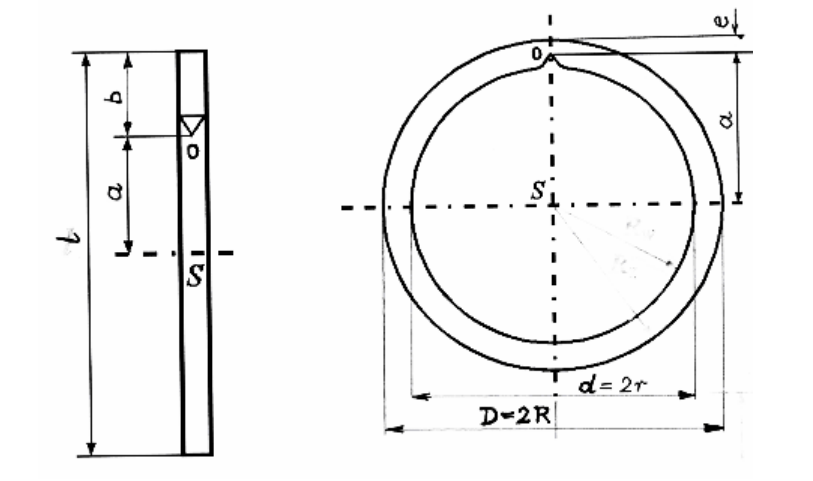
\includegraphics[width=0.7\linewidth]{./schemat}
\end{figure}

\section{Przebieg doświadczenia}

\subsection{Pomiary mas i wymiarów pręta i pierścienia oraz wyznaczenie ich okresów drgań}
\begin{enumerate}
\item Wyznaczenie masy pręta i pierścienia za pomocą wagi elektronicznej.
\item Mierzenie pręta i pierścienia wg instrukcji na rysunku {\ref{rys:1}}.
\item Umieszczenie pręta na statywie i wprawienie go w ruch drgający o małej amplitudzie.
\item Przy użyciu stopera zmierzenie czasu dwudziestu pełnych drgań.
\item Powtórzenie czynności z punktu 4 dziesięciokrotnie.
\item Policzenie okresu dla pojedynczych prób (dzieląc wyniki przez 20).
\item Policzenie średniego okresu $T_{\text{śr}}$ korzystając z wyznaczonych okresów pojedynczych prób.
\item Powtórzenie czynności od 3 do 7 dla pierścienia. 
\end{enumerate}
 
\subsection{Opracowanie wyników pomiarów}

\begin{table}[ht]
\label{table:1}
\centering
\setlength{\extrarowheight}{2pt}
\caption{\textbf{Pomiar masy i długości pręta.}}
\begin{tabular}{| @{\hspace{8mm}}c @{\hspace{8mm}}| @{\hspace{8mm}}c @{\hspace{8mm}}|@{\hspace{8mm}} c@{\hspace{8mm}}|}
\hline
 & wartość & niepewność  \\ \hline
$m[g]$ & 663 & 1 \\ \hline
$l[mm]$ & 757 & 1 \\ \hline
$b[mm]$ & 100 & 1 \\ \hline
$a[mm]$ & 275 & 1 \\ \hline

\end{tabular}
\end{table}

\begin{table}[ht]
\label{table:2}
\centering
\setlength{\extrarowheight}{2pt}
\caption{\textbf{Pomiar masy i długości pierścienia.}}
\begin{tabular}{| @{\hspace{8mm}}c @{\hspace{8mm}}| @{\hspace{8mm}}c @{\hspace{8mm}}|@{\hspace{8mm}} c@{\hspace{8mm}}|}
\hline
 & wartość & niepewność  \\ \hline
$m[g]$ & 1360 & 1 \\ \hline
$D_{W}[mm]$ & 250 & 0,1 \\ \hline
$D_{Z}[mm]$ & 280 & 1 \\ \hline
$R_{W}[mm]$ & 125 & 0,1 \\ \hline
$R_{Z}[mm]$ & 140 & 1 \\ \hline
$e[mm]$ & 10 & 0,1 \\ \hline
$a[mm]$ & 130 & 0,1 \\ \hline

\end{tabular}
\end{table}

\begin{table}[ht]
\vspace*{0.5 cm}
\centering
\setlength{\extrarowheight}{2pt}
\caption{\textbf{Pomiar okresu drgań dla pręta.}}
\label{table:okres1}
\begin{tabular}{|c|c|c|c|}
\hline
Lp. & liczba okresów $k$ & czas $t[s]$ dla $k$ okresów & okres $T_{i}$ [$s$] \\ \hline
1 & 20 & 26,73 & 1,337\\ \hline
2 & 20 & 26,98 & 1,349\\ \hline
3 & 20 & 26,73 & 1,337\\ \hline
4 & 20 & 26,83 & 1,342\\ \hline
5 & 20 & 26,95 & 1,348\\ \hline
6 & 20 & 26,67 & 1,334\\ \hline
7 & 20 & 26,77 & 1,339\\ \hline
8 & 20 & 26,80 & 1,359\\ \hline
9 & 20 & 26,67 & 1,334\\ \hline
10 & 20 & 26,80 & 1,340\\ \hline
\multicolumn{4}{|l|}{Wartość średnia okresu: $T_{\text{śr}} \colon $ 1,342 [$s$]} \\ \hline
\multicolumn{4}{|l|}{Niepewność: $u(T_{\text{śr}})\approx$  0,002490 [$s$]} \\ \hline
\end{tabular}


\end{table}

\begin{table}[!ht]
\vspace*{0.5 cm}
\centering
\setlength{\extrarowheight}{2pt}
\caption{\textbf{Pomiar okresu drgań dla pierścienia.}}
\begin{tabular}{|c|c|c|c|}
\hline
Lp. & liczba okresów $k$ & czas $t[s]$ dla $k$ okresów & okres $T_{i}$[$s$] \\ \hline
1 & 20 & 20,71 & 1,036\\ \hline
2 & 20 & 20,37 & 1,019\\ \hline
3 & 20 & 19,79 & 0,9895\\ \hline
4 & 20 & 20,59 & 1,030\\ \hline
5 & 20 & 20,68 & 1,034\\ \hline
6 & 20 & 20,65 & 1,033\\ \hline
7 & 20 & 20,45 & 1,023\\ \hline
8 & 20 & 20,37 & 1,019\\ \hline
9 & 20 & 19,72 & 0,9860\\ \hline
10 & 20 & 19,99 & 0,9995\\ \hline
\multicolumn{4}{|l|}{Wartość średnia okresu: $T_{\text{śr}} \colon $  1,017 [$s$] }\\ \hline
\multicolumn{4}{|l|} {Niepewność: $u(T{\text{śr}})\approx $ 0,005908 [$s$]}  \\ \hline
\end{tabular}
\end{table}

\subsection{Obliczenie momentu bezwładności}
\subsubsection{Obliczenie momentu bezwładności $I_{0}$ względem rzeczywistej osi obrotu korzystając z~wzoru na okres drgań}
Wzór na okres drgań wyraża się wzorem:
\begin{equation}
\label{wzor:T}
T=2\pi\sqrt{\dfrac{I_{0}}{mga}}
\end{equation}

\indent Przekształcając odpowiednio powyższe równanie {\ref{wzor:T}} otrzymujemy wzór na moment bezwładności:
\begin{equation}
I_{0}=\dfrac{mgaT^{2}}{4\pi^{2}}
\end{equation}

gdzie 
\begin{description}
\item[$m$] masa bryły [$kg$]
\item [$g$] przyspieszenie ziemskie $\left[\frac{m}{s^{2}}\right]$
\item [$T$] okres drgań [$s$] 
\item [$a$] odległość środka masy od osi obrotu [$m$]
\end{description}

\textbf{Moment bezwładności $I_{0}$ dla pręta:}
\begin{equation}
I_{0} = \dfrac{0,663\cdot 9,811 \cdot 0,275 \cdot (1,342)^{2}}{4\pi^{2}}\approx ~0,07793 \left[kg \cdot m^{2}\right]
\end{equation}

\textbf{Moment bezwładności $I_{0}$ dla pierścienia:}
\begin{equation}
I_{0} = \dfrac{1,36\cdot 9,811\cdot 0,13 \cdot (1,017)^{2}}{4\pi^{2}}\approx 0,04545~ \left[kg \cdot m^{2}\right]
\end{equation}

\subsubsection{Obliczenie momentu bezwładności $I_{S}$ względem osi przechodzącej przez środek masy korzystając z twierdzenia Steinera}
\indent Twierdzenie Steinera stosuje się do obliczania momentu bezwładności bryły względem osi przesuniętej równolegle o długość $a$, gdzie $I_{S}$ to moment bezwładności względem osi przechodzącej przez środek masy bryły.
\begin{equation}
I_{0}=I_{S}+ma^{2}
I_{S}=I_{0}-ma^{2}
\end{equation}

\textbf{Moment bezwładności $I_{S}$ dla pręta:}
\begin{equation}
I_{S} =0,07793 - 0,663 \cdot (0,275)^{2}\approx 0,03006 ~ \left[kg \cdot m^{2}\right]
\end{equation}

\textbf{Moment bezwładności $I_{S}$ dla pierścienia:}
\begin{equation}
I_{S} = 0,04545 - 1,36 \cdot (0,13)^{2}\approx 0,02298 ~ \left[kg \cdot m^{2}\right]
\end{equation}


\subsubsection{Moment bezwładności względem osi przechodzącej przez środek masy $I_{S}^{(geom)}$ na podstawie masy i wymiarów geometrycznych}
\indent Moment bezwładności większości regularnych brył można zapisać w postaci:
\begin{equation}
I_{S}^{(geom)} = k \cdot m \cdot l
\end{equation} 

gdzie 
\begin{description}
\item [$m$] masa bryły [$kg$]
\item [$l$] charakterystyczny wymiar bryły (np. długość, promień) [$m$]
\item [$k$] bezwymiarowy współczynnik zależny tylko od kształtu bryły i wyboru charakterystycznego wymiaru (np. promień czy średnica), a niezależny od wielkości bryły.
\end{description}

\textbf{Moment bezwładności $I_{S}^{(geom)}$ dla pręta:}
\begin{equation}
I_{S}^{(geom)} = \dfrac{1}{12}ml^{2}
\end{equation}
\begin{equation}
I_{S}^{(geom)} = \dfrac{1}{12}\cdot 0,663 \cdot (0,757)^{2}\approx 0,03627 ~ \left[kg \cdot m^{2}\right]
\end{equation}

\textbf{Moment bezwładności $I_{S}^{(geom)}$ dla pierścienia:}
\begin{equation}
I_{S}^{(geom)} = \dfrac{1}{12}m(R^{2}+r^{2})
\end{equation}
\begin{equation}
I_{S}^{(geom)} = \dfrac{1}{12}\cdot 1,360 \cdot ((0,140)^{2}+(0,125)^{2})\approx 0,02396 \left[kg \cdot m^{2}\right]
\end{equation}

\section{Wyznaczenie niepewności mierzonych wielkości}
\subsection{Niepewność pomiaru okresu -- niepewność typu A}
Wzór na niepewność pomiaru $u(T)$:
\begin{equation}
u(T)=\displaystyle \frac{\sqrt{\frac{\sum(T_{i}-T_{\text{śr}})^{2}}{n-1}}}{\sqrt{n}}=\displaystyle \sqrt{\frac{\sum(T_{i}-\overline{T})^{2}}{n(n-1)}}
\end{equation}

gdzie 
\begin{description}
\item [$n$] liczba pomiarów
\item [$T_{\text{śr}}$] średni czas trwania okresu  [$s$]
\end{description}

\textbf{Niepewność pomiaru okresu dla pręta:}
\begin{equation}
u(T) =\displaystyle \sqrt{\frac{(1,337-1,342)^{2} + \cdots + (1,340 - 1,342)^2}{10(10-1)}}
\end{equation}
$$u(T)\approx 0,002490 [s]$$

\textbf{Niepewność pomiaru okresu dla pierścienia:}
\begin{equation}
u(T) =\displaystyle \sqrt{\frac{(1,036-1,017)^{2} + \cdots + (0,995 - 1,017)^2}{10(10-1)}}
\end{equation}

$$u(T) \approx 0,005908 [s]$$

\subsection{Niepewność pomiaru masy}
\indent Do określenia masy pręta i pierścienia posłużyła nam waga cyfrowa o dokładności $0,001kg$, więc $u(m)=1 g$.

\subsection{Niepewność pomiaru wymiarów geometrycznych}
\indent W pomiarze pręta przyjmujemy niepewność równą działce elementarnej linijki $u(l)=1mm$, $u(a)=1mm$, $u(b)=1mm$.
\indent Zewnętrzny promień pierścienia został wyznaczony za pomocą linijki więc  $u(D_{Z})= 1mm$ i $u(R_{Z})= 1mm$> Wewnętrzny promień został wyznaczony na podstawie zewnętrznego promienia i suwmiarki, której dokładność wynosiła $o,1mm$ zatem $u(D_{W})= 0,1mm$ i $u(R_{W})= 0,1mm$. Długości tj $e$ i $a$ zostały wyznaczono z pomocą suwmiarki więc $u(e)=0,1mm$, $u(a)=0,1mm$.
%Wszystkie wartości długości związanych z pierścieniem były mierzone za pomocą suwmiarki, której %dokładność wynosiła $0,1mm$, zatem $u(D_{W})=0,1mm$, $u(D_{Z})=0,1mm$, $u(R_{W})=0,1mm$, $u(R_{Z})=0,1mm%%$, $u(e)=0,1mm$, $u(a)=0,1mm$.

\subsection{Niepewność złożona momentów bezwładności}
\subsubsection{Niepewność złożona momentu bezwładności $I_{0}$}
Wzór z którego korzystamy:
\begin{equation}
\frac{u(I_{0})}{I_{0}}=\sqrt{\left (\frac{u(m)}{m}\right ) ^2+\left ( \frac{u(a)}{a}\right )^2+\left (2 \cdot \frac{u(T)}{T}\right )^2}
\end{equation}
gdzie
\begin{description}
\item [$u(I_{0})$] niepewność pomiaru momentu bezwładności względem rzeczywistej osi obrotu
\item [$I_{0}$] moment bezwładności względem rzeczywistej osi obrotu $\left[ kg \cdot m^{2} \right]$
\item [$u(m)$] niepewność pomiaru masy
\item [$u(a)$] niepewność pomiaru odległości od środka ciężkości
\item [$u(T)$] niepewność pomiaru okresu drgań
\item [$m$] masa ciała [$kg$]
\item [$a$] odległość od środka ciężkości [$m$]
\end{description}

\textbf{Niepewność złożona momentu bezwładności $I_{0}$ dla pręta:}
\begin{equation}
\frac{u(I_{0})}{I_{0}}=\sqrt{\left(\frac{0,001}{0,663}\right) ^2+\left( \frac{0,001}{0,275}\right)^2+\left(2 \cdot \frac{0,00249}{1,342}\right)^2} \approx 0,005410 [~kg\cdot m^2]
\end{equation}

$$ u(I_{0}) \approx 0,0004216 \left[ kg \cdot m^2 \right]$$

\textbf{Niepewność złożona momentu bezwładności $I_{0}$ dla pierścienia:}
\begin{equation}
\frac{u(I_{0})}{I_{0}}=\sqrt{\left(\frac{0,001}{1,360}\right) ^2+\left( \frac{0,00001}{0,130}\right)^2+\left(2 \cdot \frac{0,005908}{1,017}\right)^2} \approx 0,01167 [~kg\cdot m^2]
\end{equation}
$$ u(I_{0}) \approx 0,0005303 \left[ kg \cdot m^2 \right]$$
\subsubsection{Niepewność złożona momentu bezwładności $I_{S}$}
Wzór z którego korzystamy:
\begin{equation}
u(I_{S})=\sqrt{\left( u(I_{0})\right)^2+\left(a^2u(m) \right)^2+\left( -2amu(m)\right)^2}
\end{equation}
gdzie
\begin{description}
\item [$I_{S}$]  moment bezwładności względem osi przechodzącej przez środek masy obliczony z wykorzystaniem twierdzenia Steinera $\left[kg \cdot m^{2} \right]$
\item [$ u(I_{S})$] niepewność momentu bezwładności względem osi przechodzącej przez środek masy obliczony z wykorzystaniem twierdzenia Steinera

\end{description}

\textbf{Niepewność złożona momentu bezwładności $I_{S}$ dla pręta:}
\begin{equation}
u(I_{S})=\sqrt{\left( 0,0004216\right)^2+\left(0,275)^2\cdot (0,001 \right)^2+\left( -2\cdot 0,0,275\cdot 0,0,663\cdot 0,001\right)^2}~\approx 0,0005625 ~[kg\cdot m^2]
\end{equation}

\textbf{Niepewność złożona momentu bezwładności $I_{S}$ dla pierścienia:}
\begin{equation}
u(I_{S})=\sqrt{\left( 0,0005303 \right)^2+\left(0,130)^2\cdot (0,0,001 \right)^2+\left( -2\cdot 0,130\cdot 1,360\cdot 0,001 \right)^2}~ \approx 0,0006376 ~ [kg\cdot m^2]
\end{equation}


\subsubsection{Niepewność złożona momentu bezwładności $I_{S}^{\text{geom}}$}
\textbf{Niepewność złożona momentu bezwładności $I_{S}^{\text{geom}}$ dla pręta:}
\begin{equation}
u(I_{s}^{\text{geom}})=\sqrt{\left(\frac{l^2}{12}\cdot u(m) \right)^2+\left(\frac{2lm}{12}\cdot u(l) \right)^2}
\approx 0,0001048 ~ [kg\cdot m^2]
\end{equation}
gdzie 
\begin{description}
\item [$I_{S}^{\text{geom}}$] moment bezwładności względem osi przechodzącej przez środek masy na podstawie masy i wymiarów geometrycznych ciała $\left[kg \cdot m^{2} \right]$
\item [$u(I_{S}^{\text{geom}})$] niepewność momentu bezwładności względem osi przechodzącej przez środek masy na podstawie masy i wymiarów geometrycznych ciała 
\end{description}

\textbf{Niepewność złożona momentu bezwładności $I_{S}^{\text{geom}}$ dla pierścienia:}
\begin{equation}
u(I_{S}^{\text{geom}})=\sqrt{\left (\frac{R_z^2+R_w^2}{2}\cdot u(m) \right )^2+\left (mR_z\cdot u(R_z) \right )^2+\left (mR_w\cdot u(R_w) \right )^2} \approx 0,0001920 ~[kg\cdot m^2]
\end{equation}

\begin{table}[ht]
\caption{\textbf{Wyniki obliczeń momentu bezwładności dla pręta.}}
\label{tab:5}
\centering
\begin{tabular}{|c|m{30mm}|m{30mm}|m{30mm}|}
\hline
& \begin{center}
\textbf{$I_{0}$ wyznaczone z~okresu drgań $[kg\cdot m^{2}]$}
\end{center} & \begin{center}
\textbf{$I_{S}$ wyznaczone z~twierdzenia Steinera $[kg\cdot m^{2}]$}
\end{center} & \begin{center}
\textbf{$I_{S}^{\text{geom}}$ wyznaczone z~pomiarów geometrycznych $[kg\cdot m^{2}]$}
\end{center}  \\ \hline
wartość & \begin{center} 0,07793\end{center} & \begin{center}0,03006\end{center} & \begin{center}0,03627\end{center}\\ \hline
niepewność &\begin{center} 0,0004216\end{center} & \begin{center}0,0005625\end{center} & \begin{center} 0,0001048 \end{center}\\ \hline

\end{tabular}
\end{table}

\begin{table}[ht]
\caption{\textbf{Wyniki obliczeń momentu bezwładności dla pierścienia.}}
\label{tab:6}
\centering
\begin{tabular}{|c|m{30mm}|m{30mm}|m{30mm}|}
\hline
& \begin{center}
\textbf{$I_{0}$ wyznaczone z~okresu drgań $[kg\cdot m^{2}]$}
\end{center} & \begin{center}
\textbf{$I_{S}$ wyznaczone z~twierdzenia Steinera $[kg\cdot m^{2}]$}
\end{center} & \begin{center}
\textbf{$I_{S}^{\text{geom}}$ wyznaczone z~pomiarów geometrycznych $[kg\cdot m^{2}]$}
\end{center}  \\ \hline
wartość & \begin{center}0,04545\end{center} & \begin{center}0,02298\end{center} & \begin{center}0,02396\end{center}\\ \hline
niepewność &\begin{center} 0,0005303\end{center} & \begin{center}0,0006376\end{center} & \begin{center}0,0001920\end{center}\\ \hline
\end{tabular}
\end{table}

\subsection{Porównanie metod wyznaczenia momentu bezwładności}
Na podstawie wartości z tabel {\ref{tab:5}} i {\ref{tab:6}} można stwierdzić, że dokładniejsze wartości momentu bezwładności uzyskuje się poprzez pomiary wymiarów geometrycznych, ponieważ niepewności pomiarów są mniejsze.

\subsection{Zgodność wyników pomiaru w granicach niepewności rozszerzonej}
Aby wyniki były zgodne w granicach niepewności rozszerzonej to 
\begin{equation}
\left|I_{S} - I_{S}^{\text{geom}}\right|<U(I_{S} - I_{S}^{\text{geom}})
\end{equation}

gdzie 
\begin{description}
\item [$I_{S}$] moment bezwładności wzgłedem osi przechodzącej przez środek masy obliczony z wykorzystaniem twierdzenia Steinera $\left[kg \cdot m^{2} \right]$
\item [$I_{S}^{\text{geom}}$] moment bezwładności obliczony na podstawie masy i wymiarów geometrycznych ciała $\left[kg \cdot m^{2} \right]$
\item [$U_(I_{S})$] niepewność $I_{S}$ $\left[kg \cdot m^{2} \right]$
\end{description}

\begin{equation}
U(I_{S} - I_{S}^{\text{geom}}) = k \cdot \sqrt{(u(I_{S})^2 + u(I_{S}^{\text{geom}})^2}
\end{equation}

gdzie 
\begin{description}
\item [$k$] współczynnik rozszerzalności równy 2
\end{description} 

\textbf{Zgodność wyników pomiaru w granicach niepewności rozszerzonej dla pręta:}

$$U(I_{s} - I_{S}^{\text{geom}}) \approx 0,001144~[kg \cdot m^2]$$
$$\left|I_{s} - I_{S}^{\text{geom}}\right| \approx 0,00621 ~[kg \cdot m^2]$$

Wyniki pomiarów uznajemy za niezgodne ze sobą, ponieważ: 
$$0,00621 > 0,001144 $$
$$\left|I_{S} - I_{S}^{\text{geom}}\right| > U(I_{s} - I_{S}^{\text{geom}})$$

\textbf{Zgodność wyników pomiaru w granicach niepewności rozszerzonej dla pierścienia:}
$$U(I_{s} - I_{S}^{\text{geom}}) \approx 0,001332 ~[kg \cdot m^2]$$
$$\left|I_{s} - I_{S}^{\text{geom}}\right| \approx 0,00098~[kg \cdot m^2]$$
Wyniki pomiarów uznajemy za niezgodne ze sobą, ponieważ: 
$$ 0,0098 > 0,001332 $$
$$\left|I_{s} - I_{S}^{\text{geom}}\right| > U(I_{s} - I_{geom})$$

\section{Wnioski}
\begin{itemize}
%\item Doświadczenie zostało przeprowadzone prawidłowo, wyniki pomiarów mieszczą się w granicach niepewności rozszerzonej zarówno dla pręta, jak i dla pierścienia.
\item Mimo przepprowadzenia doświadczenia prawidłowo wyniki pomiarów nie mieszczą sie w granicach niepewności rozszerzonej. Przyczyną może być niedokładność wymiarów pręta i pierścienia.
\item Dokładniejszym sposobem wyznaczania momentu bezwładności bryły jest skorzystanie z~zależności geometrycznych zamiast z twierdzenia Steinera.
\item Twierdzenie Steinera pozwala nam obliczyć momenty bezwładności wobec osi których nie możemy wyliczyć doświadczalnie.

\end{itemize}
\end{document}